\documentclass{article}

\usepackage[heading=true]{ctex}
\usepackage{graphicx}
\usepackage{float}
\usepackage{amsmath}
\usepackage{geometry}

\ctexset{
    section={
        number=\chinese{section},
        format+=\raggedright
    }
}
\geometry{a4paper, scale=0.7}

\begin{document}

\begin{center}
    \quad \vspace{3cm} \\
    \Large
    哈尔滨工业大学计算机科学与技术学院 \\
    
    \Huge
    实验报告 \\
    \quad \vspace{1cm} \\
    
    \Large
    \begin{tabular}{r@{:}l}
        课程名称 & 机器学习 \\
        课程类型 & 必修 \\
        实验题目 & PCA模型 \\
    \end{tabular}
    \quad \vspace{1cm} \\
    
    \large
    \begin{tabular}{r@{:}l}
    学号 & 1190200703 \\
    姓名 & 管健男 \\
    \end{tabular}

\end{center}


\section{实验目的}

掌握最小二乘法求解(无惩罚项的损失函数)、掌握加惩罚项(2范数)的损失函数优化、梯度下降法、共轭梯度法、理解过拟合、克服过拟合的方法(如加惩罚项、增加样本)。


\section{实验要求及实验环境}

\subsection{实验要求}

1. 生成数据,加入噪声;

2. 用高阶多项式函数拟合曲线;

3. 用解析解求解两种loss的最优解(无正则项和有正则项)

4. 优化方法求解最优解(梯度下降,共轭梯度);

5. 用你得到的实验数据,解释过拟合。

6. 用不同数据量,不同超参数,不同的多项式阶数,比较实验效果。

7. 语言不限,可以用matlab,python。求解解析解时可以利用现成的矩阵求逆。梯度下降,共轭梯度要求自己求梯度,迭代优化自己写。不许用现成的平台,例如pytorch,tensorflow的自动微分工具。

\subsection{实验环境}

python(numpy + matplotlib)


\section{设计思想(本程序中的用到的主要算法及数据结构)}

\subsection{PCA降维}

我们有一组数据,其中有$N$个$D$维向量$\mathbf{x}_1, \mathbf{x}_2, \ldots \mathbf{x}_N$,我们的目标是将这个数据集投影到维度$M$中去,其中$M\leq D$。

引入$D$维空间中的一组单位正交基向量
\begin{equation*}
    \begin{bmatrix}
        \mathbf{u}_1 \\
        \vdots \\
        \mathbf{u}_D \\
    \end{bmatrix}
\end{equation*}
由于是基向量,所以每个数据点都可以表示为基向量的线性组合,即
\begin{equation}
    \mathbf{x}_n=\sum^D_{i=1}\alpha_{ni}\mathbf{u}_i
    \label{alpha}
\end{equation}
其中系数$\alpha_{ni}$相当于数据点$\mathbf{x}_n$映射到以$\mathbf{u}_i$为新坐标系时的新坐标,即$\mathbf{x}_n$到基向量$\mathbf{u}_i$的投影是$\alpha_{ni}$,因此可得
\begin{equation}
    \alpha_{ni}=\mathbf{x}^T_n\mathbf{u}_i
\end{equation}
将其带入到式\ref{alpha}中,可得
\begin{equation}
    \mathbf{x}_n=\sum^D_{i=1}\left(\mathbf{x}^T_n\mathbf{u}_i\right)\mathbf{u}_i
    \label{xn}
\end{equation}

式\ref{xn}是对于向量$\mathbf{x}_n$的精准描述,但是由于我们要将$D$维降至$M$维,因此只能使用$M$个变量来描述这个$\mathbf{x}_n$。不妨用前$M$个基向量来表示这个$M$维空间,则数据点$\mathbf{x}_n$的估计值为
\begin{equation}
    \tilde{\mathbf{x}}_n = \sum^M_{i=1}z_{ni}\mathbf{u}_i + \sum^D_{i=M+1}b_i\mathbf{u}_i
    \label{txn}
\end{equation}
其中$z_{ni}$是降维后的数据点在$M$维空间中的坐标,而$b_i$是常数,对所有数据点都相同,这起到了降维的效果,数据的失真也是这一项引起的。

我们可以认为失真是真实样本与降维后的样本之间的距离。将每个样本的失真取平均,可得总体的失真,即
\begin{equation}
    J=\dfrac{1}{N}\sum^N_{n=1}\left\lVert \mathbf{x}_n-\tilde{\mathbf{x}}_n\right\rVert ^2
    \label{loss}
\end{equation}
要最小化这个失真,首先对$z_{ni}$求导
\begin{align}
    \dfrac{\partial J}{\partial z_{ni}}
    \label{lossdz}
    &= \dfrac{\partial}{\partial z_{ni}}\left(\dfrac{1}{N}\sum^N_{n=1}\left\lVert \mathbf{x}_n-\tilde{\mathbf{x}}_n\right\rVert ^2\right) \\
    &= \dfrac{\partial}{\partial z_{ni}}\left(\dfrac{1}{N}\sum^N_{n=1}\left\lVert \mathbf{x}_n-\sum^M_{i=1}z_{ni}\mathbf{u}_i-\sum^D_{i=M+1}b_i\mathbf{u}_i\right\rVert ^2\right) \\
    &= \dfrac{\partial}{\partial z_{ni}}\left(\dfrac{1}{N}\sum^N_{n=1}\left(\mathbf{x}_n-\sum^M_{i=1}z_{ni}\mathbf{u}_i-\sum^D_{i=M+1}b_i\mathbf{u}_i\right)^T\left(\mathbf{x}_n-\sum^M_{i=1}z_{ni}\mathbf{u}_i-\sum^D_{i=M+1}b_i\mathbf{u}_i\right)\right) \\
    &= \dfrac{\partial}{\partial z_{ni}}\left(\dfrac{1}{N}\sum^N_{n=1}\left(\mathbf{x}^T_n-\sum^M_{i=1}z_{ni}\mathbf{u}^T_i-\sum^D_{i=M+1}b_i\mathbf{u}^T_i\right)\left(\mathbf{x}_n-\sum^M_{i=1}z_{ni}\mathbf{u}_i-\sum^D_{i=M+1}b_i\mathbf{u}_i\right)\right) \\
    &= \dfrac{1}{N}\sum^N_{n=1}\dfrac{\partial\left(\left(\mathbf{x}^T_n-z_{ni}\mathbf{u}^T_i\right)\left(\mathbf{x}_n-z_{ni}\mathbf{u}_i\right)\right)}{\partial z_{ni}} \\
    &= \dfrac{1}{N}\sum^N_{n=1}\left(-\mathbf{x}^T_n\mathbf{u}_i-\mathbf{u}^T_i\mathbf{x}_n+2z_{ni}\mathbf{u}^T_i\mathbf{u}_i\right)
\end{align}
由于$\mathbf{u}_1, \ldots, \mathbf{u}_D$是一组单位正交基向量,所以$\mathbf{u}^T_i\mathbf{u}_i=1$。因此令式\ref{lossdz}为$0$,可得
\begin{equation}
    z_{ni}=\mathbf{x}^T_n\mathbf{u}_i
    \label{z}
\end{equation}
同理,令$J$关于$b_i$的导数为$0$,可得
\begin{equation}
    b_i=\overline{\mathbf{x}}^T\mathbf{u}_i
    \label{b}
\end{equation}
其中$\overline{\mathbf{x}}$是样本向量的均值。

利用式\ref{z}和\ref{b},代入到式\ref{txn}中,并用式\ref{xn}相减,可得
\begin{equation}
    \mathbf{x}_n-\tilde{\mathbf{x}}_n=\sum^D_{i=M+1}\left(\left(\mathbf{x}_n-\overline{\mathbf{x}}\right)^T\mathbf{u}_i\right)\mathbf{u}_i
    \label{x-tx}
\end{equation}
将式\ref{x-tx}代入到式\ref{loss}中,可得
\begin{align}
    J
    &= \dfrac{1}{N}\sum^N_{n=1}\left\lVert\mathbf{x}_n-\tilde{\mathbf{x}}_n\right\rVert ^2 \\
    &= \dfrac{1}{N}\sum^N_{n=1}\left\lVert\sum^D_{i=M+1}\left(\left(\mathbf{x}_n-\overline{\mathbf{x}}\right)^T\mathbf{u}_i\right)\mathbf{u}_i\right\rVert ^2 \\
    &= \dfrac{1}{N}\sum^N_{n=1}\left(\left(\sum^D_{i=M+1}\left(\left(\mathbf{x}_n-\overline{\mathbf{x}}\right)^T\mathbf{u}_i\right)\mathbf{u}_i\right)^T\left(\sum^D_{i=M+1}\left(\left(\mathbf{x}_n-\overline{\mathbf{x}}\right)^T\mathbf{u}_i\right)\mathbf{u}_i\right)\right) \\
    &= \dfrac{1}{N}\sum^N_{n=1}\left(\left(\sum^D_{i=M+1}\left(\left(\mathbf{x}_n-\overline{\mathbf{x}}\right)^T\mathbf{u}_i\right)\mathbf{u}^T_i\right)\left(\sum^D_{i=M+1}\left(\left(\mathbf{x}_n-\overline{\mathbf{x}}\right)^T\mathbf{u}_i\right)\mathbf{u}_i\right)\right)
\end{align}
由于$\mathbf{u}_1, \ldots, \mathbf{u}_D$是一组单位正交基向量,所以$\mathbf{u}^T_i\mathbf{u}_i=1$且$\mathbf{u}^T_i\mathbf{u}_j=0$,因此上式可继续化简
\begin{align}
    J
    &= \dfrac{1}{N}\sum^N_{n=1}\left(\sum^D_{i=M+1}\left(\left(\left(\mathbf{x}_n-\overline{\mathbf{x}}\right)^T\mathbf{u}_i\right)\left(\left(\mathbf{x}_n-\overline{\mathbf{x}}\right)^T\mathbf{u}_i\right)\right)\right) \\
    &= \dfrac{1}{N}\sum^N_{n=1}\left(\sum^D_{i=M+1}\left(\left(\left(\mathbf{x}_n-\overline{\mathbf{x}}\right)^T\mathbf{u}_i\right)^T\left(\left(\mathbf{x}_n-\overline{\mathbf{x}}\right)^T\mathbf{u}_i\right)\right)\right) \\
    &= \dfrac{1}{N}\sum^N_{n=1}\left(\sum^D_{i=M+1}\left(\left(\mathbf{u}^T_i\left(\mathbf{x}_n-\overline{\mathbf{x}}\right)\right)\left(\left(\mathbf{x}_n-\overline{\mathbf{x}}\right)^T\mathbf{u}_i\right)\right)\right) \\
    &= \dfrac{1}{N}\sum^N_{n=1}\left(\sum^D_{i=M+1}\left(\mathbf{u}^T_i\left(\mathbf{x}_n-\overline{\mathbf{x}}\right)\left(\mathbf{x}_n-\overline{\mathbf{x}}\right)^T\mathbf{u}_i\right)\right) \\
    &= \sum^D_{i=M+1}\left(\mathbf{u}^T_i\left(\dfrac{1}{N}\sum^N_{n=1}\left(\mathbf{x}_n-\overline{\mathbf{x}}\right)\left(\mathbf{x}_n-\overline{\mathbf{x}}\right)^T\right)\mathbf{u}_i\right) \\
    &= \sum^D_{i=M+1}\mathbf{u}^T_i\mathbf{S}\mathbf{u}_i
\end{align}
其中
\begin{equation}
    \mathbf{S}=\dfrac{1}{N}\sum^N_{n=1}\left(\mathbf{x}_n-\overline{\mathbf{x}}\right)\left(\mathbf{x}_n-\overline{\mathbf{x}}\right)^T
\end{equation}
正是样本数据向量的协方差矩阵。

要在一个方向$\mathbf{u}_i$上,针对$J$进行最小化。考虑到约束条件$\mathbf{u}^T_i\mathbf{u}_i=1$,可用拉格朗日乘子法,对$\mathbf{u}_i$求导
\begin{align}
    \dfrac{\partial\mathcal{L}}{\partial\mathbf{u}_i}
    &= \dfrac{\partial}{\partial\mathbf{u}_i}\left(\mathbf{u}^T_i\mathbf{S}\mathbf{u}_i+\lambda_i\left(1-\mathbf{u}^T_i\mathbf{u}_i\right)\right) \\
    &= 2\left(\mathbf{S}\mathbf{u}_i-\lambda_i\mathbf{u}_i\right)
\end{align}
令其为$0$,可得
\begin{equation}
    \mathbf{S}\mathbf{u}_i=\lambda_i\mathbf{u}_i
    \label{S}
\end{equation}
可见$\mathbf{u}_i$一定是$\mathbf{S}$的一个特征向量。在式\ref{S}的两侧左乘$\mathbf{u}^T_i$,因此可得
\begin{equation}
    \lambda_i=\mathbf{u}^T_i\mathbf{S}\mathbf{u}_i
\end{equation}
所以
\begin{align}
    J
    &= \sum^D_{i=M+1}\mathbf{u}^T_i\mathbf{S}\mathbf{u}_i \\
    &= \sum^D_{i=M+1}\lambda_i
\end{align}

因此,只需选择$D-M$个最小的特征值对应的特征向量,就可以获得$J$的最小值;而剩余的$M$个较大特征值的特征向量则对应了降维后的$M$维空间的基向量。

\subsection{数据旋转}

数据降维是针对$M<D$的情景。而当$M=D$时,仅仅是将坐标轴旋转,将计算得到的特征向量作为新的坐标系的基向量。

\subsection{数据重建}

在式\ref{xn}的基础上,对每个数据点进行平移,可得
\begin{equation}
    \overline{\mathbf{x}}_n=\sum^D_{i=1}\left(\overline{\mathbf{x}}^T_n\mathbf{u}_i\right)\mathbf{u}_i
\end{equation}
再将式\ref{z}和\ref{b}代入式\ref{txn}中,可得用$M$维数据重建回$D$维的公式
\begin{align}
    \tilde{\mathbf{x}}_n
    &= \sum^M_{i=1}\left(\mathbf{x}^T_n\mathbf{u}_i\right)\mathbf{u}_i+\sum^D_{i=M+1}\left(\overline{\mathbf{x}}^T\mathbf{u}_i\right)\mathbf{u}_i \\
    &= \sum^M_{i=1}\left(\mathbf{x}^T_n\mathbf{u}_i\right)\mathbf{u}_i+\sum^D_{i=1}\left(\overline{\mathbf{x}}^T\mathbf{u}_i\right)\mathbf{u}_i-\sum^M_{i=1}\left(\overline{\mathbf{x}}^T\mathbf{u}_i\right)\mathbf{u}_i \\
    &= \overline{\mathbf{x}}+\sum^M_{i=1}\left(\mathbf{x}^T_n\mathbf{u}_i-\overline{\mathbf{x}}^T\mathbf{u}_i\right)\mathbf{u}_i
\end{align}


\section{实验结果与分析}

\subsection{生成数据}

为了保证生成的数据满足朴素贝叶斯假设,$raw\_data()$函数保证相同类别的向量$\mathbf{X}^l$,其各个维度都有
\begin{eqnarray}
    x^l_i \sim \mathcal{N} \left(\mu, \sigma\right)
\end{eqnarray}
即各个维度$x^l_i$都服从各自的正态分布。

生成的两类数据如图\ref{gen_data}。

\begin{figure}[htbp]
    \centering
    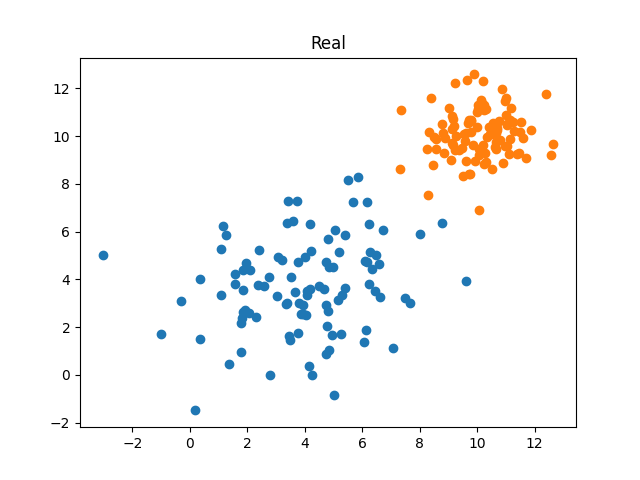
\includegraphics[width=0.7\textwidth]{figures/Figure_1.png}
    \caption{生成两类数据}
    \label{gen_data}
\end{figure}

\subsection{梯度下降法确定分类面}

使用梯度下降法迭代$10000$次,确定分类面系数$\mathbf{w}$,从而获得了分类面方程
\begin{equation}
    \label{sep_equ}
    \mathbf{w}^T\mathbf{X}=0
\end{equation}

对于一个二维向量的原始数据,方程\ref{sep_equ}也可写为
\begin{equation}
    w_0 + w_1 x + w_2 y = 0
\end{equation}
由此可以作出二维平面上的分类面图像,如图\ref{sep_equ_figure}。

\begin{figure}[htbp]
    \centering
    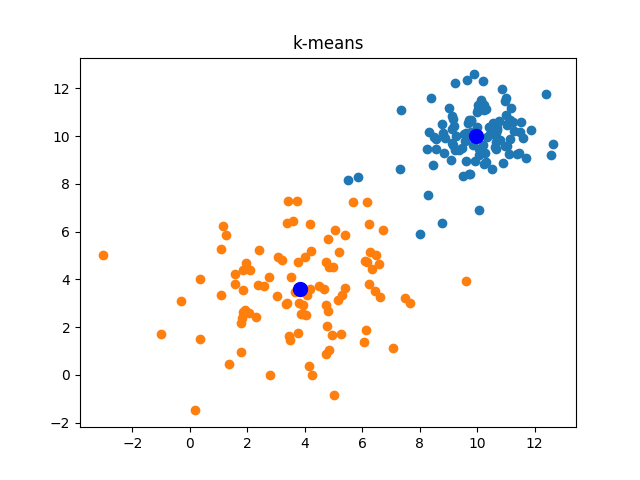
\includegraphics[width=0.7\textwidth]{figures/Figure_2.png}
    \caption{分类面}
    \label{sep_equ_figure}
\end{figure}

绘制出分类面后,同样可以计算分类误差。计算方式为
\begin{equation}
    loss = \dfrac{count_{01}}{count_0}
\end{equation}
即:类别$0$的点,分到类别$1$的个数$/$类别$0$的点的总个数

图\ref{sep_equ_figure}所示的分类面,其分类所需的迭代次数及误差如图\ref{loss}

\begin{figure}[htbp]
    \centering
    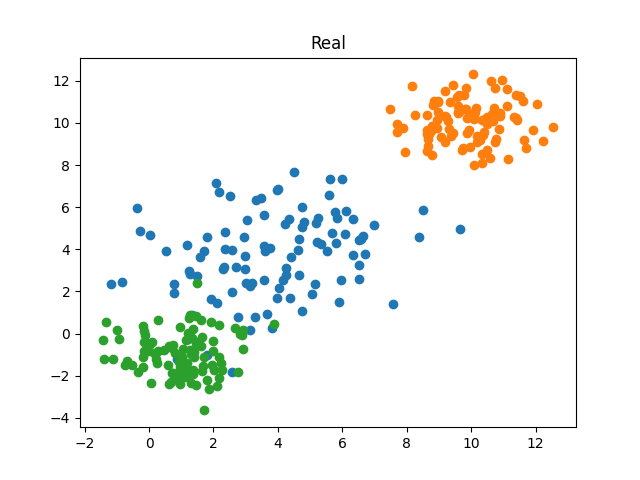
\includegraphics[width=0.7\textwidth]{figures/Figure_3.png}
    \caption{分类面误差}
    \label{loss}
\end{figure}

\subsection{溢出问题}

在进行梯度下降迭代的过程中,常常会出现Numpy警报Overflow的情况,如图\ref{overflow}。

\begin{figure}[htbp]
    \centering
    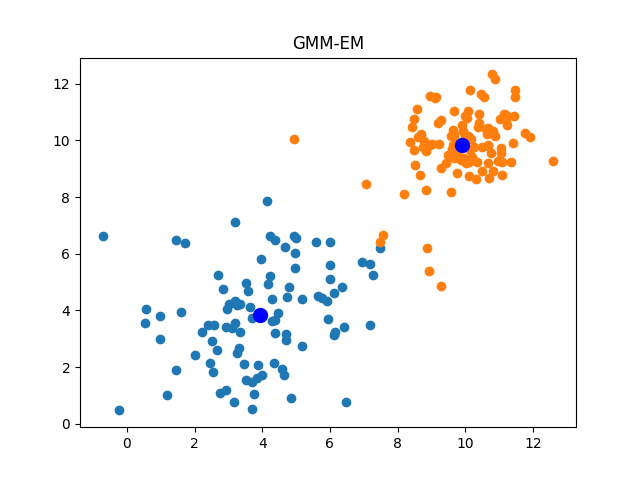
\includegraphics[width=0.7\textwidth]{figures/Figure_9.png}
    \caption{Numpy警报Overflow}
    \label{overflow}
\end{figure}

分析这一现象产生的原因。这个问题是由于在计算式\ref{gd_final}中的$\exp\left(\mathbf{w}^T\mathbf{X}\right)$时,由于$\mathbf{w}^T\mathbf{X}$较大,导致计算出的指数函数过大溢出\cite{overflow}。解决方法是在数学上做一些变形:对于式\ref{gd_final},当$\exp\left(\mathbf{w}^T\mathbf{X}^l\right)=\infty$时,式\ref{gd_final}可进一步化简
\begin{align}
    \mathbf{w}_{k+1}
    &= \mathbf{w}_k+\alpha\left(\sum^L_{l=1}\mathbf{X}^l\left(Y^l-\dfrac{\exp\left(\mathbf{w}^T\mathbf{X}^l\right)}{1+\exp\left(\mathbf{w}^T\mathbf{X}^l\right)}\right)-\lambda\mathbf{w}\right) \\
    &= \mathbf{w}_k+\alpha\left(\sum^L_{l=1}\mathbf{X}^l\left(Y^l-1\right)-\lambda\mathbf{w}\right)
\end{align}

上述变形并没有完全解决问题。考虑当$\mathbf{w}^T\mathbf{X}<0$时,若其绝对值较大,可能会使$\exp\left(\mathbf{w}^T\mathbf{X}\right)$过于趋近$0$而导致下溢,因此仍需进一步变形,即
\begin{align}
    \mathbf{w}_{k+1}
    &= \mathbf{w}_k+\alpha\left(\sum^L_{l=1}\mathbf{X}^l\left(Y^l-\dfrac{\exp\left(\mathbf{w}^T\mathbf{X}^l\right)}{1+\exp\left(\mathbf{w}^T\mathbf{X}^l\right)}\right)-\lambda\mathbf{w}\right) \\
    &= \mathbf{w}_k+\alpha\left(\sum^L_{l=1}\mathbf{X}^l\left(Y^l-\dfrac{1}{\exp\left(-\mathbf{w}^T\mathbf{X}^l\right)+1}\right)-\lambda\mathbf{w}\right)
\end{align}

上述变形的代码如下

\rule{\textwidth}{0.01em}
\begin{verbatim}
    for (X, Y) in data:
        wx = np.dot(np.transpose(w), X)
        if wx >= 0:
            expwx = np.exp(wx)
            if expwx == np.inf:
                sum_l += (Y - 1) * np.array(X)
            else:
                sum_l += (Y - expwx / (1 + expwx)) * np.array(X)
        else:
            expnwx = np.exp(-wx)
            if expnwx == np.inf:
                sum_l += Y * np.array(X)
            else:
                sum_l += (Y - 1 / (expnwx + 1)) * np.array(X)
    w = w + alpha * (sum_l - lam * w)
\end{verbatim}
\rule{\textwidth}{0.01em}

\subsection{加入正则项}

对于逻辑回归的
\begin{equation}
    \mathbf{w}^T\mathbf{X}=0
\end{equation}
的分类面的形式,对于实验中的2维向量并不会出现过拟合现象。因此在此处加入正则项只是简化了模型的复杂度。

采取与实验一类似的方式,从一个较小的值开始依次计算正则项系数$\lambda$可能取到的值,比较各自的loss,从而选取一个最合适的$\lambda$。

图\ref{lambda20}和图\ref{lambda100}分别展示了样本数据量为$40$和$100$时、$\lambda$为$0.01$时的分类效果(如图中红色直线所示)。绿色直线为不加入正则项,而红色直线为加入正则项,图中可见二者几乎重叠,因此在此处是否加入正则项对分类的精度几乎无影响。

\begin{figure}[htbp]
    \begin{minipage}[t]{0.5\linewidth}
        \centering
        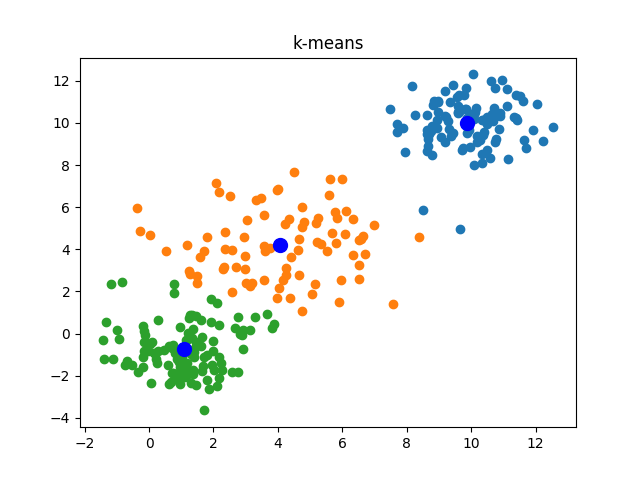
\includegraphics[width=\textwidth]{figures/Figure_4.png}
        \caption{每个类别的样本数量为$20$时的情况}
        \label{lambda20}
    \end{minipage}
    \begin{minipage}[t]{0.5\linewidth}
        \centering
        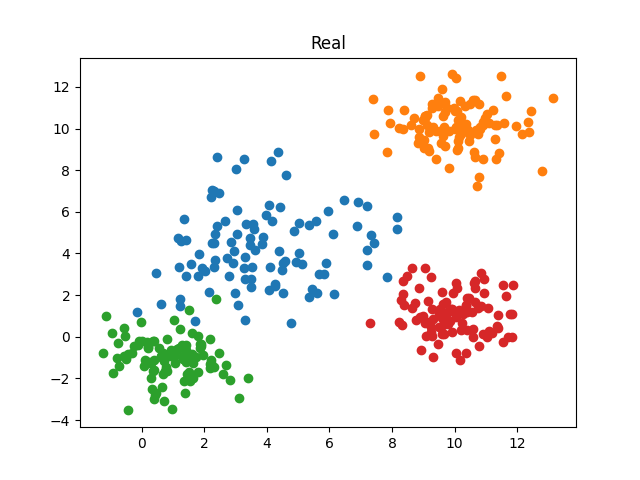
\includegraphics[width=\textwidth]{figures/Figure_5.png}
        \caption{每个类别的样本数量为$100$时的情况}
        \label{lambda100}
    \end{minipage}
\end{figure}

\subsection{破坏朴素贝叶斯假设}

破坏生成的数据中的朴素贝叶斯假设。$raw\_data\_dim2()$保证向量的第一个维度(即$x$)服从正态分布,而第二个维度(即$y$)是一个值与$x$的差,这样$x$和$y$的相关系数就是$-1$。绘制原始数据和分类面,如图\ref{no-native}。

\begin{figure}[htbp]
    \begin{minipage}[t]{0.5\linewidth}
        \centering
        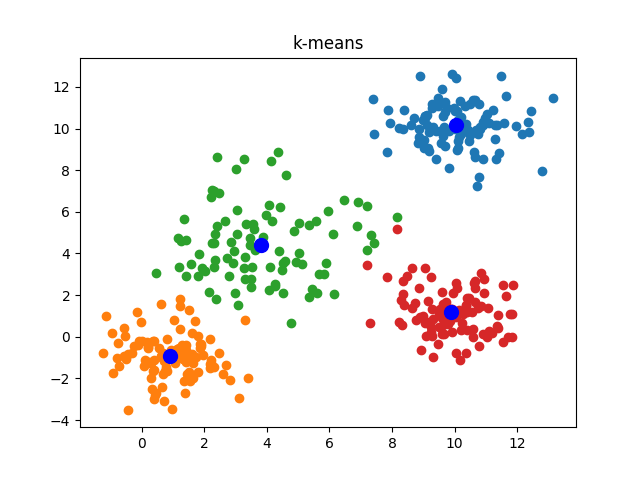
\includegraphics[width=\textwidth]{figures/Figure_6.png}
        \caption{不满足朴素贝叶斯假设的原始数据,使用逻辑回归进行分类}
        \label{no-native}
    \end{minipage}
    \begin{minipage}[t]{0.5\linewidth}
        \centering
        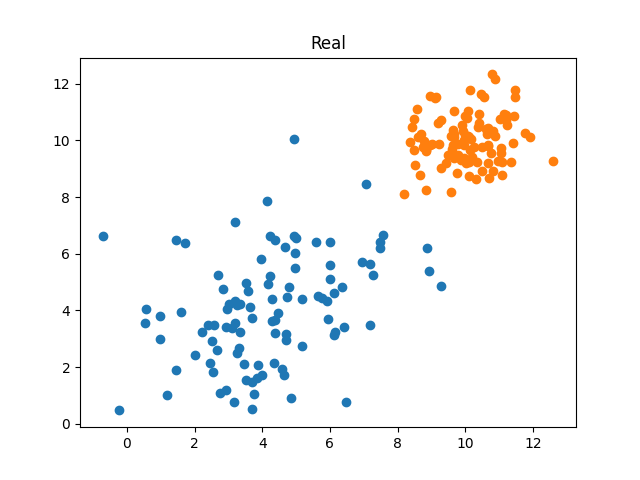
\includegraphics[width=\textwidth]{figures/Figure_7.png}
        \caption{不满足朴素贝叶斯假设的分类误差。其中第一个loss是不含正则项的误差,第二个loss是带有正则项的误差}
        \label{no-native-loss}
    \end{minipage}
\end{figure}

分类后的误差如图\ref{no-native-loss},与图\ref{loss}相比,分类效果并不好。

\subsection{UCI网站数据分类}

使用的数据为钞票数据集Banknote Dataset\cite{uci}。这是从纸币鉴别过程中的图像里提取的数据,用来预测钞票的真伪的数据集。样本中的每一行有5个数值,分别是4个输入和1个输出,其意义分别为:

第一列:图像经小波变换后的方差

第二列:图像经小波变换后的偏态

第三列:图像经小波变换后的峰度

第四列:图像的熵

第五列:钞票所属的类别(0或1)。

因此,在逻辑回归中,上述样本的前四项可以看作是一个4维向量,而最后一列则是这个向量的类别。使用逻辑回归对给定的样本进行分类,由于4维向量不便于展示,此处仅给出分类的误差分析,如图\ref{uci}。

\begin{figure}[htbp]
    \centering
    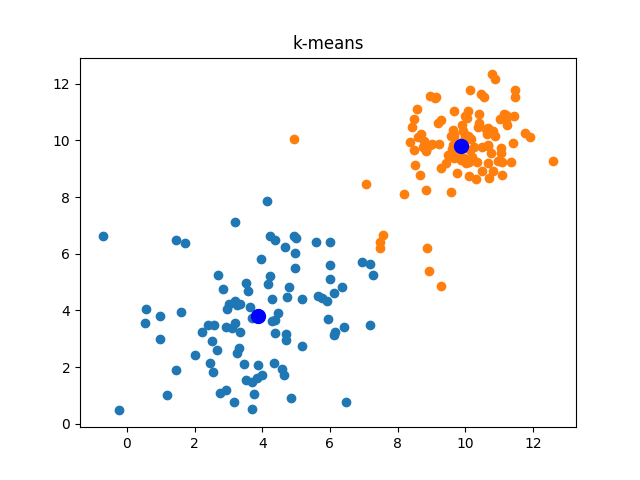
\includegraphics[width=0.7\textwidth]{figures/Figure_8.png}
    \caption{使用逻辑回归对UCI钞票数据集进行分类的误差}
    \label{uci}
\end{figure}

可见分类效果良好。


\section{结论}

对于梯度下降法,是否使用惩罚项对于测试结果的影响不大。

对于满足朴素贝叶斯假设的数据,使用逻辑回归进行分类的效果比较好;但是对于不符合朴素贝叶斯假设的数据,逻辑回归虽然准确率下降,但是依然能够在一定程度上进行正确分类\cite{no-native}。


\begin{thebibliography}{99}

\end{thebibliography}


\appendix

\section{附录:源代码(带注释)}

\begin{verbatim}
import numpy as np
import matplotlib.pyplot as plt


def gauss_vector(mu_list: float, sigma_list: float, dim: int = 2) -> list:
    """生成一个向量,其各个维度服从正态分布

    Args:
        mu_list:    正态分布均值,其中 mu_list[i] 是第 i 维的均值
        sigma_list: 正态分布方差,其中 sigma_list[i] 是第 i 维的方差
        dim:        向量维数

    Returns:
        返回向量
    """

    vector = []
    for i in range(0, dim):
        vector.append(np.random.normal(mu_list[i], sigma_list[i], 1)[0])

    return vector


def raw_data(count: int, mu_list: list, sigma_list: list, dim: int = 2) -> list:
    """生成 count 组向量
    向量的维度是 dim 维,各个维度服从正态分布,
    其中 mu_list[i] 是第 i 维的均值,sigma_list[i] 是第 i 维的方差

    Args:
        count:      向量组数
        mu_list:    正态分布均值
        sigma_list: 正态分布方差
        dim:        向量维数

    Returns:
        返回一个 list,包含 count 个向量
    """

    vector_list = []
    for i in range(0, count):
        vector_list.append(gauss_vector(mu_list, sigma_list, dim))

    return vector_list


def raw_data_dim2(count: int, mu: float, sigma: float, weight: float) -> list:
    """生成 count 组 2 维向量,
    其 x 维度服从正态分布,均值是 mu,方差是 sigma;
    其 y 维度与 x 维度的和是 (weight * 一个 (0, 1) 内的随机数)

    Args:
        count:  向量组数
        mu:     正态分布均值
        sigma:  正态分布方差
        weight: 两个维度的和的权重

    Returns:
        返回一个 list,包含 count 个 2 维向量
    """

    vector_list = []
    for i in range(0, count):
        vector = [np.random.normal(mu, sigma, 1)[0]]
        vector.append(weight * np.random.random() - vector[0])
        vector_list.append(vector)

    return vector_list


def draw_line(w: list, start: int, stop: int, label: str, color: str) -> None:
    """绘制直线
    w = [w0, w1, w2],绘制的直线为 w1 * x + w2 * y + w0 = 0,
    即 y = - 1/w2 * (w1 * x + w0)


    Args:
        w:     直线方程参数
        start: 起始横坐标
        stop:  终止横坐标
        label: 图例
        color: 颜色
    """

    x_list = np.arange(start, stop, step=0.01)
    y_list = (-1 / w[2]) * (w[1] * x_list + w[0])

    plt.plot(x_list, y_list, c=color, label=label)


def insert_one(vectors: list) -> list:
    """向一组向量中,每个向量的首部都加一个 1
    [
        [1, x1, x2, ...],
        ...,
        [1, z1, z2, ...],
    ]

    Args:
        vectors: 一个向量组成的 list

    Returns:
        返回添加 1 的向量组
    """

    new_vectors = []
    for vec in vectors:
        new_vectors.append([1] + vec)

    return new_vectors


def select_dim(vectors: list, dim: int) -> list:
    """将一组向量中的第 dim 维的坐标提取出来,放入一个 list

    Args:
        vectors: 向量
        dim:     需要提取的维数

    Returns:
        返回第 dim 维坐标组成的列表
    """

    index_list = []
    for vec in vectors:
        index_list.append(vec[dim])

    return index_list


def tidy_data(vectors: list, classes: list) -> list:
    """整理数据,生成的格式为:
    [
        [vector0, class],
        [vector1, class],
        ...,
        [vectorn, class]
    ]
    其中每个 class 为对应 vector 的类别号

    Args:
        vectors: 向量列表
        classes: 类别列表,classes[i] 是 vectors[i] 的类别

    Returns:
        返回整理后的数据
    """

    data = []
    for i in range(0, len(classes)):
        data.append([vectors[i], classes[i]])

    return data


def calc_loss(data: list, w: list) -> float:
    """计算分类面的误差
    误差定义为:类别 0 的点,分到类别 1 的个数 / 类别 0 的点的总个数

    Args:
        data: 训练数据
        w:    分类面系数

    Returns:
        返回误差
    """

    class0_count = 0
    error_count = 0
    for vec in data:
        X = vec[0]
        Y = vec[1]
        if Y == 0:
            # 统计类别 0 的点的总个数
            class0_count += 1
        if np.dot(np.transpose(w), X) < 0 and Y == 1:
            # X 被分到类别 0,但是实际上 X 是类别 1
            error_count += 1

    return error_count / class0_count


def gd(
    data: list, dim: int, lam: float, alpha: float = 0.01, max_turn: int = 10000
) -> list:
    """梯度下降法求分类面系数

    Args:
        data:     分类的数据列表
        dim:      向量维度数
        alpha:    学习率
        lam:      正则项系数
        max_turn: 最大迭代次数

    Returns:
        返回分类面的系数
    """

    turn = 0

    w = np.ones(dim + 1)
    while True:
        sum_l = 0
        for vec in data:
            X = vec[0]
            Y = vec[1]
            expwx = np.exp(np.dot(np.transpose(w), X))
            sum_l += (Y - expwx / (1 + expwx)) * np.array(X)
        w = w + alpha * (sum_l + lam * w)

        turn += 1
        if turn >= max_turn:
            print("===== hit max_turn limit =====")
            print("loss = " + str(calc_loss(data, w)))
            break

    print("turn = " + str(turn))
    return w


def load_data(filename: str, dim: int) -> list:
    """从文件中加载数据
    文件格式必须为
    x0,x1,...,xn,c0
    ...,
    x0,x1,...,xn,cm
    其中每一行的前 dim 个数据为训练数据向量的各个维度,最后一个数据为此行数据的类别

    Args:
        filename: 文件名
        dim:      数据维度

    Returns:
        返回加载的数据
    """

    result = []
    with open(filename, "r") as f:
        for line in f:
            data_line = [float(i) for i in line.removesuffix("\n").split(",")]
            vec = data_line[:-1]
            class_id = int(data_line[-1])
            result.append([[1] + vec, class_id])

    return result


if __name__ == "__main__":
    # 从文件中加载数据
    # data = load_data("lab2/data_banknote_authentication.txt", 4)
    # w = gd(data, dim=4, lam=0)
    # calc_loss(data, w)
    # exit(0)

    class0_count = 20
    class1_count = 20

    # 满足朴素贝叶斯假设的原始数据
    class0_vector = raw_data(class0_count, [1, 1], [1, 1])
    class1_vector = raw_data(class1_count, [3, 3], [1, 1])

    # 不满足朴素贝叶斯假设的原始数据
    # class0_vector = raw_data_dim2(class0_count, 1, 1, 10)
    # class1_vector = raw_data_dim2(class1_count, 3, 1, 10)

    # 对原始向量进行增广
    class0_vector_new = insert_one(class0_vector)
    class1_vector_new = insert_one(class1_vector)

    data = tidy_data(
        class0_vector_new + class1_vector_new,
        [0] * class0_count + [1] * class1_count,
    )

    # ===== 绘图 =====

    plt.title("Lab 2")

    # 类别 0
    class0_x_list = select_dim(class0_vector, 0)
    class0_y_list = select_dim(class0_vector, 1)
    plt.scatter(class0_x_list, class0_y_list, label="class 0")

    # 类别 1
    class1_x_list = select_dim(class1_vector, 0)
    class1_y_list = select_dim(class1_vector, 1)
    plt.scatter(class1_x_list, class1_y_list, label="class 1")

    # 分类面
    w = gd(data, dim=2, lam=0)
    draw_line(w, start=-1, stop=5, label="gd", color="g")
    w = gd(data, dim=2, lam=0.01)
    draw_line(w, start=-1, stop=5, label="gd lambda", color="r")

    plt.legend()
    plt.show()

\end{verbatim}


\end{document}
